% erstellt mit https://www.mathcha.io/editor

\begin{center}
    



    \tikzset{every picture/.style={line width=0.75pt}} %set default line width to 0.75pt        

    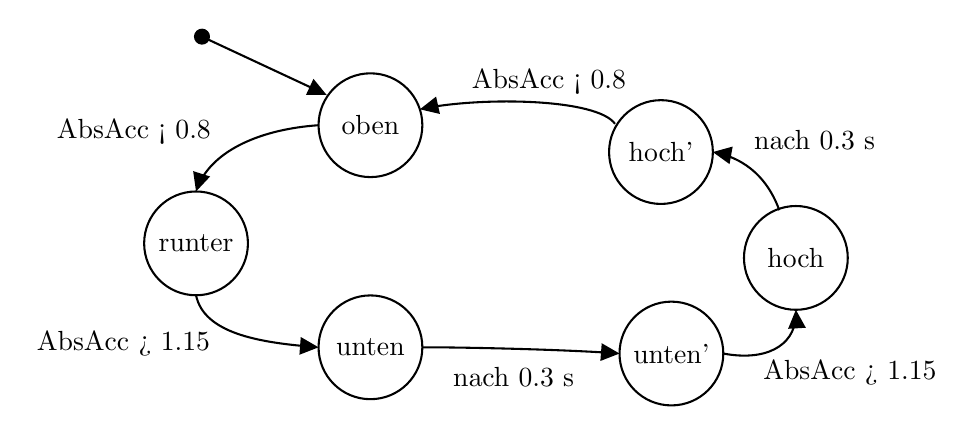
\begin{tikzpicture}[x=0.75pt,y=0.75pt,yscale=-1,xscale=1]
    %uncomment if require: \path (0,612.0170516967773); %set diagram left start at 0, and has height of 612.0170516967773
    
    %Shape: Circle [id:dp4115012649218517] 
    \draw   (172,454) .. controls (172,440.19) and (183.19,429) .. (197,429) .. controls (210.81,429) and (222,440.19) .. (222,454) .. controls (222,467.81) and (210.81,479) .. (197,479) .. controls (183.19,479) and (172,467.81) .. (172,454) -- cycle ;
    %Straight Lines [id:da06931047169438798] 
    \draw    (115.83,411.33) -- (173.11,438.06) ;
    \draw [shift={(175.83,439.33)}, rotate = 205.02] [fill={rgb, 255:red, 0; green, 0; blue, 0 }  ][line width=0.08]  [draw opacity=0] (8.93,-4.29) -- (0,0) -- (8.93,4.29) -- cycle    ;
    \draw [shift={(115.83,411.33)}, rotate = 25.02] [color={rgb, 255:red, 0; green, 0; blue, 0 }  ][fill={rgb, 255:red, 0; green, 0; blue, 0 }  ][line width=0.75]      (0, 0) circle [x radius= 3.35, y radius= 3.35]   ;
    %Shape: Circle [id:dp48735130026263906] 
    \draw   (87.97,510.93) .. controls (87.97,497.12) and (99.17,485.93) .. (112.97,485.93) .. controls (126.78,485.93) and (137.97,497.12) .. (137.97,510.93) .. controls (137.97,524.74) and (126.78,535.93) .. (112.97,535.93) .. controls (99.17,535.93) and (87.97,524.74) .. (87.97,510.93) -- cycle ;
    %Curve Lines [id:da6609208305880534] 
    \draw    (172,454) .. controls (144.45,455.9) and (121.39,465.86) .. (114.01,483.14) ;
    \draw [shift={(112.97,485.93)}, rotate = 287.53] [fill={rgb, 255:red, 0; green, 0; blue, 0 }  ][line width=0.08]  [draw opacity=0] (8.93,-4.29) -- (0,0) -- (8.93,4.29) -- cycle    ;
    
    %Shape: Circle [id:dp9177005648524454] 
    \draw   (172,561) .. controls (172,547.19) and (183.19,536) .. (197,536) .. controls (210.81,536) and (222,547.19) .. (222,561) .. controls (222,574.81) and (210.81,586) .. (197,586) .. controls (183.19,586) and (172,574.81) .. (172,561) -- cycle ;
    %Curve Lines [id:da8997751532087288] 
    \draw    (112.97,535.93) .. controls (116.81,554.2) and (143.04,558.63) .. (169.16,560.77) ;
    \draw [shift={(172,561)}, rotate = 184.38] [fill={rgb, 255:red, 0; green, 0; blue, 0 }  ][line width=0.08]  [draw opacity=0] (8.93,-4.29) -- (0,0) -- (8.93,4.29) -- cycle    ;
    
    %Shape: Circle [id:dp5913276051851417] 
    \draw   (317,564) .. controls (317,550.19) and (328.19,539) .. (342,539) .. controls (355.81,539) and (367,550.19) .. (367,564) .. controls (367,577.81) and (355.81,589) .. (342,589) .. controls (328.19,589) and (317,577.81) .. (317,564) -- cycle ;
    %Curve Lines [id:da588437346756167] 
    \draw    (222,561) .. controls (237.42,560.93) and (286.38,561.86) .. (314.07,563.79) ;
    \draw [shift={(317,564)}, rotate = 184.38] [fill={rgb, 255:red, 0; green, 0; blue, 0 }  ][line width=0.08]  [draw opacity=0] (8.93,-4.29) -- (0,0) -- (8.93,4.29) -- cycle    ;
    
    %Shape: Circle [id:dp9891196847216435] 
    \draw   (376.97,517.93) .. controls (376.97,504.12) and (388.17,492.93) .. (401.97,492.93) .. controls (415.78,492.93) and (426.97,504.12) .. (426.97,517.93) .. controls (426.97,531.74) and (415.78,542.93) .. (401.97,542.93) .. controls (388.17,542.93) and (376.97,531.74) .. (376.97,517.93) -- cycle ;
    %Curve Lines [id:da6447447682801046] 
    \draw    (367,564) .. controls (386.74,567.76) and (401.16,560.86) .. (401.98,545.89) ;
    \draw [shift={(401.97,542.93)}, rotate = 446.63] [fill={rgb, 255:red, 0; green, 0; blue, 0 }  ][line width=0.08]  [draw opacity=0] (8.93,-4.29) -- (0,0) -- (8.93,4.29) -- cycle    ;
    
    %Curve Lines [id:da7537207989164001] 
    \draw    (314.83,453.33) .. controls (305.94,441.05) and (251.26,440.36) .. (223.34,445.81) ;
    \draw [shift={(220.83,446.33)}, rotate = 347.47] [fill={rgb, 255:red, 0; green, 0; blue, 0 }  ][line width=0.08]  [draw opacity=0] (8.93,-4.29) -- (0,0) -- (8.93,4.29) -- cycle    ;
    
    %Shape: Circle [id:dp7322215580168285] 
    \draw   (311.97,466.93) .. controls (311.97,453.12) and (323.17,441.93) .. (336.97,441.93) .. controls (350.78,441.93) and (361.97,453.12) .. (361.97,466.93) .. controls (361.97,480.74) and (350.78,491.93) .. (336.97,491.93) .. controls (323.17,491.93) and (311.97,480.74) .. (311.97,466.93) -- cycle ;
    %Curve Lines [id:da44315821397943034] 
    \draw    (393.97,494.93) .. controls (390.04,483.91) and (381.72,471.63) .. (364.73,467.51) ;
    \draw [shift={(361.97,466.93)}, rotate = 370.22] [fill={rgb, 255:red, 0; green, 0; blue, 0 }  ][line width=0.08]  [draw opacity=0] (8.93,-4.29) -- (0,0) -- (8.93,4.29) -- cycle    ;
    
    
    % Text Node
    \draw (197,454) node   [align=left] {oben};
    % Text Node
    \draw (83,457.04) node  [font=\normalsize] [align=left] {AbsAcc < 0.8};
    % Text Node
    \draw (112.97,510.93) node   [align=left] {runter};
    % Text Node
    \draw (283,433.04) node  [font=\normalsize] [align=left] {AbsAcc < 0.8};
    % Text Node
    \draw (78,559.04) node  [font=\normalsize] [align=left] {AbsAcc > 1.15};
    % Text Node
    \draw (197,561) node   [align=left] {unten};
    % Text Node
    \draw (266,575.04) node  [font=\normalsize] [align=left] {nach 0.3 s};
    % Text Node
    \draw (342,564) node   [align=left] {unten'};
    % Text Node
    \draw (428,573.04) node  [font=\normalsize] [align=left] {AbsAcc > 1.15};
    % Text Node
    \draw (401.97,517.93) node   [align=left] {hoch};
    % Text Node
    \draw (336.97,466.93) node   [align=left] {hoch'};
    % Text Node
    \draw (411,461.04) node  [font=\normalsize] [align=left] {nach 0.3 s};
    
    
    \end{tikzpicture}
    
\end{center}